\documentclass[10pt]{article}
\usepackage[utf8]{inputenc}
\usepackage{array, xcolor, bibentry}
\usepackage[margin=3cm]{geometry}

\usepackage[english]{babel}
\selectlanguage{english}

\usepackage{graphicx}
\graphicspath{ {./img/} }

\title{\bfseries M. Joaquín García González}
\author{manliojoaquin@gmail.com}
\date{}

\definecolor{lightgray}{gray}{0.8}
\newcolumntype{L}{>{\raggedleft}p{0.18\textwidth}}
\newcolumntype{R}{p{0.8\textwidth}}
\newcommand\VRule{\color{lightgray}\vrule width 0.5pt}

\begin{document}
    \pagenumbering{gobble}% Remove page numbers (and reset to 1)

    \maketitle

    \begin{minipage}[ht]{0.48\textwidth}
        Urb. Porlier, Módulo ``o'', Nº 8\\
        C/ General, Bajamar 38250\\
        San Cristóbal de La Laguna\\
        \\
        Nationality: Spanish, Argentinian\\
        Birth date: October 29th, 1990\\
        Telephone: +34 655 141 227
    \end{minipage}
    \begin{minipage}[ht]{0.48\textwidth}
        \begin{flushright}
        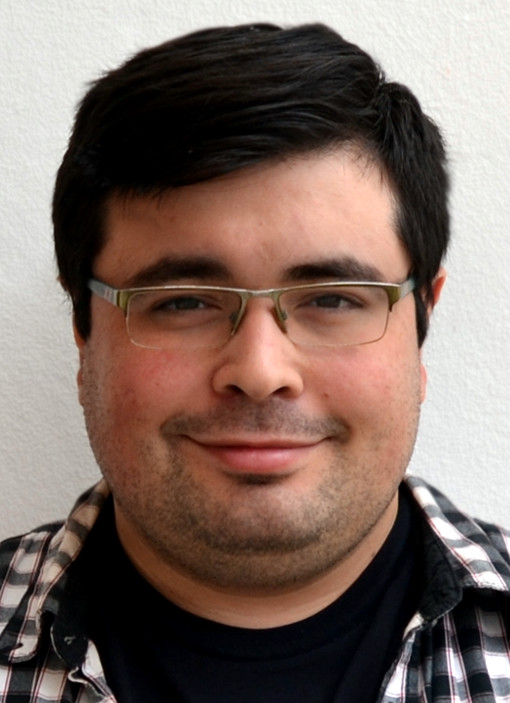
\includegraphics[height=8em]{profile}
        \end{flushright}
    \end{minipage}

    \section*{Usual tasks}
    \begin{itemize}
        \item Administration of computer equipment based on GNU-Linux and Windows.

        \item Development of web pages, mobile applications and standard software.

        \item Assembly and repair of desktop PCs, laptops and network infrastructure.

        \item Design of graphic materials, interfaces and products.
    \end{itemize}

    \section*{Programming languages}
    \begin{center}
    \begin{tabular}{ c c c c c c c c c c }

        Bash & Ruby & PHP & C\# & CSS & HTML & Javascript & \LaTeX & Unity-Script & Elixir

    \end{tabular}
    \end{center}

    \section*{Known Software}
    \begin{tabular}{L!{\VRule}R}

        Development environments&Vim, Brackets, Unity3D, Atom.\\\\

        Version control&Git.\\\\

        Collaborative tools&Telegram, Slack, Trello, IRC, Git-Hub.\\\\

        Operative systems&Android, Windows and GNU-Linux (usual administrator), OSX (occasional administrator).\\\\

        Office&MS Office, Libre Office, Open Office and \LaTeX.\\\\

        Computer aided design and image manipulation&Imagemagick, Adobe Photoshop, Adobe Ilustrator, 3D Studio, Gimp, Inkscape and others.\\\\

    \end{tabular}

    \section*{Languages}
    \begin{tabular}{L!{\VRule}R}

        Spanish&Mother tongue\\\\

        English&Fluent (B2 certificate by the official language school of La Laguna in 2009.)\\\\

    \end{tabular}

    \section*{Professional Experience}
    \begin{tabular}{L!{\VRule}R}
        2016--Now&{Independent web development.}\\\\

        2015--2016&{Administration of a computer room under the management of the Office of Free Software for the University of La Laguna.}\\\\

        2015--2016&{Technical service for the company Horizont Atlantic SL.}\\\\

        2011--2014&{Development of video games for the company 4D3 Studio.}\\\\

        2014&{Design of geolocated mobile video game ``Progrezz''}\\\\

        2014&{Collaborating member in the organization and layout of the ``XV International Congress of Human Computer Interaction 2014'', held in
        Puerto de la Cruz in September 2014}.\\\\

        2011--2012&{Collaboration in the development of the Mundo Isla video game for the University of La Laguna in the project for the promotion of healthy habits ``SAVEH''}.\\\\

        2009--2012&{Billboards for degrees of the University of La Laguna.}\\\\

    \end{tabular}

    \section*{Volunteering and Free Software}
    \begin{tabular}{L!{\VRule}R}

        2009&{Technical volunteer at the free software event ``Gran Canaria Desktop Summit''}\\\\

    \end{tabular}

    \section*{Imparted courses}
    \begin{tabular}{L!{\VRule}R}

        2014&{Speaker at the First Summer Scientific Campus in the Innovation Area of the General Foundation of the University of La Laguna.}\\\\

        2013--2014&{Computer classes at user level to individuals.}\\\\

        2013&{Professor of the workshop ``Introduction to HTML5 and CSS3'' for the General Foundation of the University of La Laguna.}\\\\

        2013&{Professor of the workshop ``Videogames Level 1: Project'' for the General Foundation of the University of La Laguna.}\\\\

        2012--2013&{Professor of robotics at Nuriana S.L. (La Laguna).}\\\\

    \end{tabular}

    \section*{Academic training}
    \begin{tabular}{L!{\VRule}R}

        Now&{\bf Currently studying: }Upper grade training cycle in the development of multiplatform applications.\\\\

        2010&Bachelor's degree with specialization in Humanities and Social Sciences. CEAD Santa Cruz de Tenerife Mercedes Pinto.\\\\

        2007--2008&Cultural exchange to Australia. Certified by AFS Intercultura.\\\\[5pt]

    \end{tabular}

    \section*{Professional training}
    \begin{tabular}{L!{\VRule}R}

        2014&Training in web programming languages and systems administration, 240 Theoretical-practical hours. Certified by Fotón Sistemas Inteligentes. September 2014.\\\\

        2011&Introduction workshop to Adobe Flash, 20 Theoretical-practical hours. Certified by the Business Foundation of the University of La Laguna. May 2011.\\\\

        2009--2010&III Course of traditional animation and cartoons, 830 Theoretical-practical hours. Certified by La Mirada Producciones. July 2010.\\\\

    \end{tabular}

    \section*{Other merits}
    \begin{tabular}{L!{\VRule}R}

        &Coauthor of the article ``Promoting and Supporting Healthy Living By Design'' in the minutes of the INTERACT 2011 conference.\\\\

    \end{tabular}

    \bibliographystyle{plain}
    \nobibliography{publication}

    {\bf\scriptsize\vfill\hfill In La Laguna, \today.}
\end{document}
